\section{Diskrete Fourier Transformation (DFT)}
	$$\boxed{s(h)=\sum_{k=0}^{N-1}\hat c_k e^{jhk\frac{2\pi}{N}}=\sum_{k=0}^{N-1}
	\left[ \hat{a}_k \cos\left(hk \frac{2 \pi}{N}\right)+\hat{b}_k \sin\left(hk
	\frac{2 \pi}{N}\right) \right]} \qquad N=\text{Periodenanzahl}$$\\
	$$\hat{c}_k=\frac{1}{N}\sum_{h=0}^{N-1}s(h)
	e^{-jhk\frac{2\pi}{N}}=\hat{a}_k-j\hat{b}_k \qquad \hat{a}_k=\frac{1}{N}
	\sum_{h=0}^{N-1}s(h) \cos\left(hk \frac{2 \pi}{N}\right)=Re(\hat{c}_k) \qquad
	\hat{b}_k=\frac{1}{N} \sum_{h=0}^{N-1}s(h) \sin\left(hk \frac{2
	\pi}{N}\right)=-Im(\hat{c}_k)$$\\	

	\subsection{Berechnung mit Matrizen}
		\textbf{Transformation}\\
		1. Periode $N$ des Signalvektors $\vec{s}=
		\begin{bmatrix}
		s(0) \\
		s(1) \\
		s(N-1)\\
		\end{bmatrix}$ bestimmen\\ \\
		2. Einheitswurzel $w$ berechnen: $w=e^{j\frac{2 \pi}{N}}$\\ \\
		3. Matrix $W$ berechnen: $W=
		\begin{bmatrix}
		w^0 & w^0 & w^0 & \ldots & w^0\\
		w^0 & w^1 & w^2 & \ldots & w^{N-1}\\
		w^0 & w^2 & w^4 & \ldots & w^{2(N-1)}\\
		\ldots & \ldots & \ldots & \ldots & \ldots\\
		w^0 & w^{N-1} & w^{2(N-1)} & \ldots & w^{(N-1)(N-1)}                        
		\end{bmatrix}$\\ \\
		4. Matrix $V$ berechnen: $V=W^*$ (konj. komplex)\\ \\
		5. Koeffizienten bzw. Fouriertransformierte $\vec{c}$ berechnen:
		$\vec{c}=\frac{1}{N}V\vec{s}$\\

		\begin{minipage}{13cm}
			\textbf{Rücktransformation}\\
			1. Matrix $W$ (wie bei der Transformation beschrieben) berechnen \\
			2. Signalvektor $\vec{s}$ berechnen: $\vec{s}=W\vec{c}$	
			\subsection{Matrizenmultiplikation}
			\begin{tabular}{ll}
				$\frac14
				\begin{bmatrix}
				    6 & -1 & 4 \\
				    3 & 2 & -2 \\
				    0 & -3 & -1
				\end{bmatrix}
				\cdot
				\begin{bmatrix}
					1 \\
				    4 \\
				    3 
				\end{bmatrix}
				=
				\frac14
				\begin{bmatrix}
					6 \cdot 1 + (-1) \cdot 4 + 4 \cdot 3\\
					3 \cdot 1 + 2 \cdot  4 + (-2) \cdot 3\\
					0 \cdot 1 + (-3) \cdot 4 + (-1) \cdot 3  
				\end{bmatrix}
				=
				\frac14
				\begin{bmatrix}
				    14\\
				    5\\
				    -15
				\end{bmatrix}
				=
				\begin{bmatrix}
		        	3.5\\
		        	1.25\\
		        	-3.75
		        \end{bmatrix}$
		    \end{tabular}		
        \end{minipage}
		\begin{minipage}[c]{5cm}
        	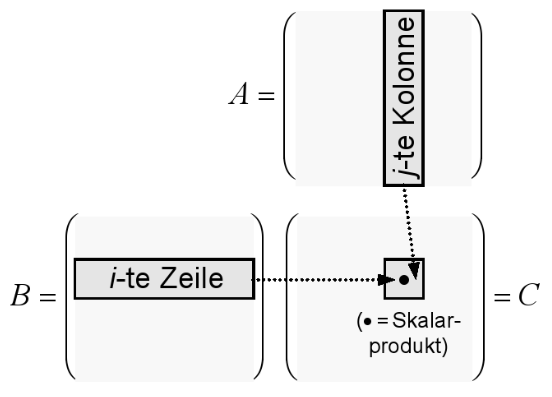
\includegraphics[width=5cm]{./bilder/matrix.png}
        \end{minipage}
		
	\subsection{Einige W-Matrizen}
		\begin{tabular}{l l l l}
        N = 2 & N = 3 & N = 4 & N = 6\\
		$\begin{bmatrix}
		1 & 1\\
		1 & -1\\              
		\end{bmatrix}$ &
		$\begin{bmatrix}
		1 & 1 & 1\\
		1 & -\frac{1}{2}+j\frac{\sqrt{3}}{2} & -\frac{1}{2}-j\frac{\sqrt{3}}{2}\\
		1 & -\frac{1}{2}-j\frac{\sqrt{3}}{2} & -\frac{1}{2}+j\frac{\sqrt{3}}{2}\\
		\end{bmatrix}$ &
		$\begin{bmatrix}
		1 & 1 & 1 & 1 \\
		1 & j & -1 & -j\\
		1 & -1 & 1 & -1\\
		1 & -j & -1 & j\\                   
		\end{bmatrix}$ &
		$\begin{bmatrix}
		1 & 1 & 1 & 1 & 1 & 1\\
		1 & \frac{1}{2}+j\frac{\sqrt{3}}{2} & -\frac{1}{2}+j\frac{\sqrt{3}}{2} & -1
		& -\frac{1}{2}-j\frac{\sqrt{3}}{2} & \frac{1}{2}-j\frac{\sqrt{3}}{2}\\
		1 & -\frac{1}{2}+j\frac{\sqrt{3}}{2} & -\frac{1}{2}-j\frac{\sqrt{3}}{2} & 1
		& -\frac{1}{2}+j\frac{\sqrt{3}}{2} & -\frac{1}{2}-j\frac{\sqrt{3}}{2}\\
		1 & -1 & 1 & -1 & 1 & -1\\
		1 & -\frac{1}{2}-j\frac{\sqrt{3}}{2} & -\frac{1}{2}+j\frac{\sqrt{3}}{2} & 1
		& -\frac{1}{2}-j\frac{\sqrt{3}}{2} & -\frac{1}{2}+j\frac{\sqrt{3}}{2}\\ 
		1 & \frac{1}{2}-j\frac{\sqrt{3}}{2} & -\frac{1}{2}-j\frac{\sqrt{3}}{2} & -1
		& -\frac{1}{2}+j\frac{\sqrt{3}}{2} & \frac{1}{2}+j\frac{\sqrt{3}}{2}\\ 
		\end{bmatrix}$
		\end{tabular}

		\begin{tabular}{l }
        N = 8\\
 		$\begin{bmatrix}
		1 & 1 & 1 & 1 & 1 & 1 & 1 & 1\\ 
		1 & \frac{\sqrt{2}}{2}+\frac{\sqrt{2}}{2}j & j &
		-\frac{\sqrt{2}}{2}+\frac{\sqrt{2}}{2}j & -1 & 
		-\frac{\sqrt{2}}{2}-\frac{\sqrt{2}}{2}j & -j & 
		\frac{\sqrt{2}}{2}-\frac{\sqrt{2}}{2}j\\
		1 & j & -1 & -j & 1 & j & -1 & -j\\
		1 &	-\frac{\sqrt{2}}{2}+\frac{\sqrt{2}}{2}j & -j & 
		\frac{\sqrt{2}}{2}+\frac{\sqrt{2}}{2}j & -1 & 
		\frac{\sqrt{2}}{2}-\frac{\sqrt{2}}{2}j & j &
		-\frac{\sqrt{2}}{2}-\frac{\sqrt{2}}{2}j\\
		1 & -1 & 1 & -1 & 1 & -1 & 1 & -1\\
		1 &	-\frac{\sqrt{2}}{2}-\frac{\sqrt{2}}{2}j & j &
		\frac{\sqrt{2}}{2}-\frac{\sqrt{2}}{2}j & -1 &
		\frac{\sqrt{2}}{2}+\frac{\sqrt{2}}{2}j & -j &
		-\frac{\sqrt{2}}{2}+\frac{\sqrt{2}}{2}j\\
		1 & -j & -1 & j & 1 & -j & -1 & j\\
		1 &	\frac{\sqrt{2}}{2}-\frac{\sqrt{2}}{2}j & -j & 
		-\frac{\sqrt{2}}{2}-\frac{\sqrt{2}}{2}j & -1 &
		-\frac{\sqrt{2}}{2}+\frac{\sqrt{2}}{2}j & j &
		\frac{\sqrt{2}}{2}+\frac{\sqrt{2}}{2}j
		\end{bmatrix}$
		\end{tabular}


	
	
	
	